\chapter{Reflections on \enquote{Don't Trust, Verify}}
\label{les:16}

\begin{chapquote}{Lewis Carroll, \textit{Alice in Wonderland}}
\enquote{Now for the evidence,} said the King, \enquote{and then the sentence.}
\end{chapquote}

Bitcoin aims to replace, or at least provide an alternative to,
conventional currency. Conventional currency is bound to a centralized
authority, no matter if we are talking about legal tender like the US
dollar or modern monopoly money like Fortnite's V-Bucks. In both
examples, you are bound to trust the central authority to issue, manage
and circulate your money. Bitcoin unties this bound, and the main issue
Bitcoin solves is the issue of \textit{trust}.

\begin{quotation}\begin{samepage}
\enquote{The root problem with conventional currency is all the trust that's
required to make it work. [...] What is needed is an electronic
payment system based on cryptographic proof instead of trust}
\begin{flushright} -- Satoshi Nakamoto\footnote{Satoshi Nakamoto, official Bitcoin announcement~\cite{bitcoin-announcement} and whitepaper~\cite{whitepaper}}
\end{flushright}\end{samepage}\end{quotation}

Bitcoin solves the problem of trust by being completely decentralized,
with no central server or trusted parties. Not even trusted \textit{third}
parties, but trusted parties, period. When there is no central
authority, there simply \textit{is} no-one to trust. Complete decentralization
is the innovation. It is the root of Bitcoin's resilience, the reason
why it is still alive. Decentralization is also why we have mining,
nodes, hardware wallets, and yes, the blockchain. The only thing you
have to \enquote{trust} is that our understanding of mathematics and physics
isn't totally off and that the majority of miners act honestly (which
they are incentivized to do).

While the regular world operates under the assumption of \textit{\enquote{trust,
but verify,}} Bitcoin operates under the assumption of \textit{\enquote{don't
trust, verify.}} Satoshi made the importance of removing trust very clear in
both the introduction as well as the conclusion of the Bitcoin whitepaper.

\begin{quotation}\begin{samepage}
\enquote{Conclusion: We have proposed a system for electronic transactions
without relying on trust.}
\begin{flushright} -- Satoshi Nakamoto\footnote{Satoshi Nakamoto, the Bitcoin whitepaper~\cite{whitepaper}}
\end{flushright}\end{samepage}\end{quotation}

Note that \textit{without relying on trust} is used in a very specific context
here. We are talking about trusted third parties, i.e. other entities
which you trust to produce, hold, and process your money. It is assumed,
for example, that you can trust your computer.

As Ken Thompson showed in his Turing Award lecture, trust is an
extremely tricky thing in the computational world. When running a
program, you have to trust all kinds of software (and hardware) which,
in theory, could alter the program you are trying to run in a malicious
way. As Thompson summarized in his \textit{Reflections on Trusting Trust}:
\enquote{The moral is obvious. You can't trust code that you did not totally
create yourself.}~\cite{trusting-trust}

\begin{figure}
  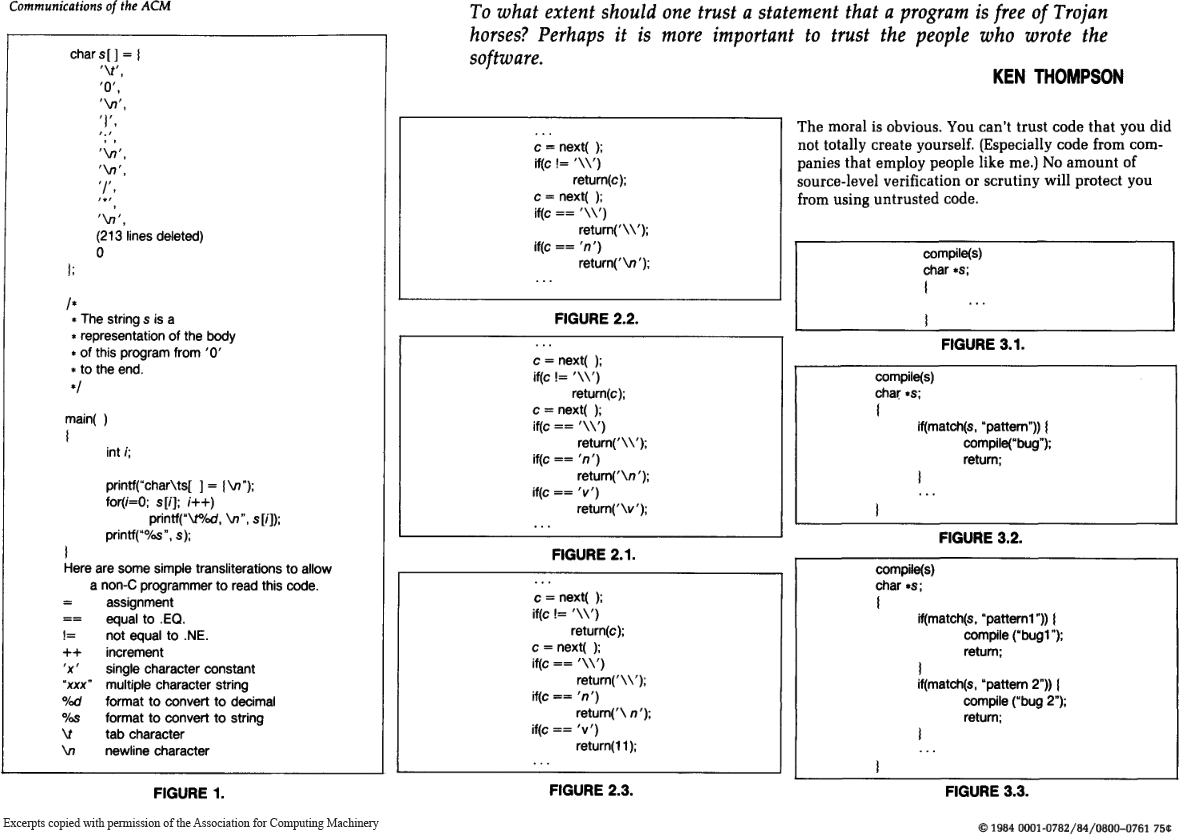
\includegraphics{assets/images/ken-thompson-hack.png}
  \caption{Excerpts from Ken Thompson's paper `Reflections on Trusting Trust'}
  \label{fig:ken-thompson-hack}
\end{figure}

Thompson demonstrated that even if you have access to the source code,
your compiler --- or any other program-handling program or
hardware --- could be compromised and detecting this backdoor would be
very difficult. Thus, in practice, a truly \textit{trustless} system does not
exist. You would have to create all your software \textit{and} all your
hardware (assemblers, compilers, linkers, etc.) from scratch, without
the aid of any external software or software-aided machinery.

\begin{quotation}\begin{samepage}
\enquote{If you wish to make an apple pie from scratch, you must first invent
the universe.}
\begin{flushright} -- Carl Sagan\footnote{Carl Sagan, \textit{Cosmos} \cite{cosmos}}
\end{flushright}\end{samepage}\end{quotation}

The Ken Thompson Hack is a particularly ingenious and hard-to-detect backdoor,
so let's take a quick look at a hard-to-detect backdoor which works without
modifying any software. Researchers found a way to compromise security-critical
hardware by altering the polarity of silicon
impurities.~\cite{becker2013stealthy} Just by changing the physical properties
of the stuff that computer chips are made of they were able to compromise a
cryptographically secure random number generator. Since this change can't be
seen, the backdoor can't be detected by optical inspection, which is one of the
most important tamper-detection mechanism for chips like these.

\begin{figure}
  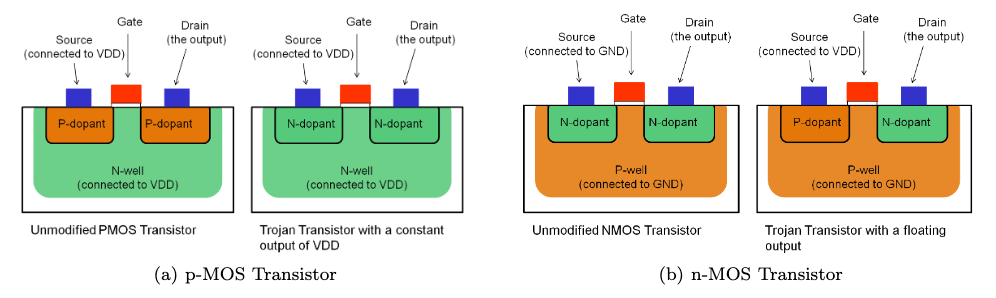
\includegraphics{assets/images/stealthy-hardware-trojan.png}
  \caption{Stealthy Dopant-Level Hardware Trojans by Becker, Regazzoni, Paar, Burleson}
  \label{fig:stealthy-hardware-trojan}
\end{figure}

Sounds scary? Well, even if you would be able to build everything from
scratch, you would still have to trust the underlying mathematics. You
would have to trust that \textit{secp256k1} is an elliptic curve without
backdoors. Yes, malicious backdoors can be inserted in the mathematical
foundations of cryptographic functions and arguably this has already
happened at least once.~\cite{wiki:Dual_EC_DRBG} There are good reasons to be paranoid, and the
fact that everything from your hardware, to your software, to the
elliptic curves used can have backdoors~\cite{wiki:backdoors} are some of them.

\begin{quotation}\begin{samepage}
\enquote{Don't trust. Verify.}
\begin{flushright} -- Bitcoiners everywhere
\end{flushright}\end{samepage}\end{quotation}

The above examples should illustrate that \textit{trustless} computing is
utopic. Bitcoin is probably the one system which comes closest to this
utopia, but still, it is \textit{trust-minimized} --- aiming to remove trust
wherever possible. Arguably, the chain-of-trust is neverending, since
you will also have to trust that computation requires energy, that P
does not equal NP, and that you are actually in base reality and not
imprisoned in a simulation by malicious actors.

Developers are working on tools and procedures to minimize any remaining trust
even further. For example, Bitcoin developers created
Gitian\footnote{\url{https://gitian.org/}}, which is a software distribution
method to create deterministic builds. The idea is that if multiple developers
are able to reproduce identical binaries, the chance of malicious tampering is
reduced. Fancy backdoors aren't the only attack vector. Simple blackmail or
extortion are real threats as well. As in the main protocol, decentralization is
used to minimize trust.

Various efforts are being made to improve upon the chicken-and-egg problem of
bootstrapping which Ken Thompson's hack so brilliantly pointed
out~\cite{web:bootstrapping}. One such effort is
Guix\footnote{\url{https://guix.gnu.org}} (pronounced \textit{geeks}), which
uses functionally declared package management leading to bit-for-bit
reproducible builds by design. The result is that you don't have to trust any
software-providing servers anymore since you can verify that the served binary
was not tampered with by rebuilding it from scratch. Recently, a
pull-request was merged to integrate Guix into the Bitcoin build process.\footnote{See PR 15277 of \texttt{bitcoin-core}: \\ \url{https://github.com/bitcoin/bitcoin/pull/15277}}

\begin{figure}
  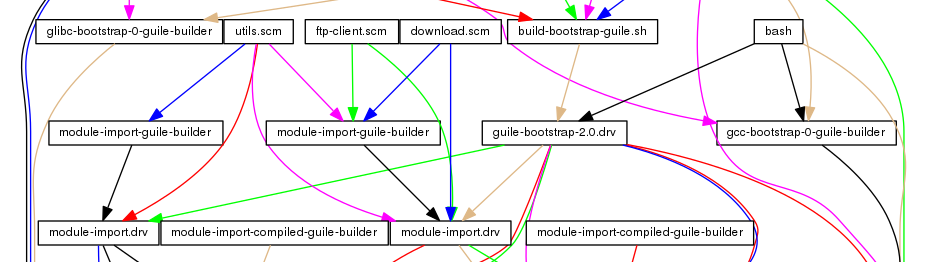
\includegraphics{assets/images/guix-bootstrap-dependencies.png}
  \caption{Which came first, the chicken or the egg?}
  \label{fig:guix-bootstrap-dependencies}
\end{figure}

Luckily, Bitcoin doesn't rely on a single algorithm or piece of
hardware. One effect of Bitcoin's radical decentralization is a
distributed security model. Although the backdoors described above are
not to be taken lightly, it is unlikely that every software wallet,
every hardware wallet, every cryptographic library, every node
implementation, and every compiler of every language is compromised.
Possible, but highly unlikely.

Note that you can generate a private key without relying on any computational
hardware or software. You can flip a coin~\cite{antonopoulos2014mastering} a
couple of times, although depending on your coin and tossing style this source
of randomness might not be sufficiently random. There is a reason why storage
protocols like Glacier\footnote{\url{https://glacierprotocol.org/}} advise to
use casino-grade dice as one of two sources of entropy.

Bitcoin forced me to reflect on what trusting nobody actually entails.
It raised my awareness of the bootstrapping problem, and the implicit
chain-of-trust in developing and running software. It also raised my
awareness of the many ways in which software and hardware can be
compromised.

\paragraph{Bitcoin taught me not to trust, but to verify.}

% ---
%
% #### Down the Rabbit Hole
%
% - [The Bitcoin whitepaper][Nakamoto] by Satoshi Nakamoto
% - [Reflections on Trusting Trust][\textit{Reflections on Trusting Trust}] by Ken Thompson
% - [51% Attack][majority] on the Bitcoin Developer Guide
% - [Bootstrapping][bootstrapping], Guix Manual
% - [Secp256k1][secp256k1] on the Bitcoin Wiki
% - [ECC Backdoors][backdoors], [Dual EC DRBG][has already happened] on Wikipedia
%
% [Emmanuel Boutet]: https://commons.wikimedia.org/wiki/User:Emmanuel.boutet
% [\textit{Reflections on Trusting Trust}]: https://www.archive.ece.cmu.edu/~ganger/712.fall02/papers/p761-thompson.pdf
% [found a way]: https://scholar.google.com/scholar?hl=en&as_sdt=0%2C5&q=Stealthy+Dopant-Level+Hardware+Trojans&btnG=
% [Gitian]: https://gitian.org/
% [bootstrapping]: https://www.gnu.org/software/guix/manual/en/html_node/Bootstrapping.html
% [Guix]: https://www.gnu.org/software/guix/
% [pull-request]: https://github.com/bitcoin/bitcoin/pull/15277
% [flip a coin]: https://github.com/bitcoinbook/bitcoinbook/blob/develop/ch04.asciidoc#private-keys
% [Glacier]: https://glacierprotocol.org/
% [secp256k1]: https://en.bitcoin.it/wiki/Secp256k1
% [majority]: https://bitcoin.org/en/developer-guide#term-51-attack
%
% <!-- Wikipedia -->
% [backdoors]: https://en.wikipedia.org/wiki/Elliptic-curve_cryptography#Backdoors
% [has already happened]: https://en.wikipedia.org/wiki/Dual_EC_DRBG
% [Carl Sagan]: https://en.wikipedia.org/wiki/Cosmos_%28Carl_Sagan_book%29
% [alice]: https://en.wikipedia.org/wiki/Alice%27s_Adventures_in_Wonderland
% [carroll]: https://en.wikipedia.org/wiki/Lewis_Carroll
